\documentclass[12pt]{report}

\usepackage{
    courier,
    algorithm,
    algpseudocode,
    listings,
    underscore,
    authblk,
    hyperref,
    tikz,
    pgfplots,
    tabularx
}

\pgfplotsset{compat=newest, width=\textwidth}
\usepgfplotslibrary{statistics}

\usetikzlibrary{positioning}

\setlength{\parindent}{0pt}

\lstset{
    basicstyle=\ttfamily\footnotesize,
    breaklines=true,
    aboveskip=15pt,
    belowskip=15pt,
}

\begin{document}

\title{RTOS Documentation}

\author{
    Kathleen Chung\\
    \texttt{kklchung@uwaterloo.ca}
    \and
    Connor Cimowsky\\
    \texttt{ccimowsky@uwaterloo.ca}
    \and
    Christian De Angelis\\
    \texttt{cdeangel@uwaterloo.ca}
    \and
    Jaclyne Ooi\\
    \texttt{jpooi@uwaterloo.ca}
}

\maketitle

\begin{abstract}

This document describes a real-time operating system for the Keil MCB1700 Evaluation Board. It examines the design of the operating system, documents user-facing primitives, and provides an analysis of system performance.

\end{abstract}

\tableofcontents

\listofalgorithms

\listoffigures

\chapter{Design Description}

\section{Operating System Initialization}

Once the operating system image has been copied to the LPC1768's on-chip ROM, execution can be initiated by pressing the \texttt{RESET} button on the MCB1700 board. The address of the \texttt{main} function is then loaded into the program counter and the CPU begins fetching and executing instructions. Subsequently, the board's hardware components (e.g., LEDs, timers, serial controllers) are initialized.

\subsection{Memory Initialization}

Now that the board's hardware is ready, it is necessary to initialize global data structures such as process control queues and the keyboard command registry. Most importantly, a portion of the on-chip SRAM is divided into fixed-size blocks (see \hyperref[app:configuration]{Appendix~\ref*{app:configuration}}) and inserted into the global memory heap.

\subsection{Process Initialization}

Upon completion of memory initialization, this procedure iterates through the process initialization table and performs three tasks. First, it populates the process control block (PCB) for each process. Next, each PCB is placed in the ready queue (unless it is an i-process, since these processes are invoked by interrupt handlers). Finally, a stack frame is allocated for each process and the resulting stack pointer is stored in its PCB. At this point, the first process can be scheduled by invoking \hyperref[alg:releasingtheprocessor]{\texttt{release_processor}}.

\section{Memory Management}

\subsection{Heap Data Structure}

Our memory heap structure is implemented using a generic linked list. Each node in the list represents a single memory block that can be requested by invoking the \hyperref[alg:requestingmemoryblocks]{\texttt{request_memory_block}} primitive and released by invoking the \hyperref[alg:releasingmemoryblocks]{\texttt{release_memory_block}} primitive. Nodes in the memory heap are spaced apart using a predefined block size (see \hyperref[app:configuration]{Appendix~\ref*{app:configuration}}).

\subsection{Requesting Memory Blocks}

When a process invokes \hyperref[alg:requestingmemoryblocks]{\texttt{request_memory_block}}, the operating system first checks if the heap is empty. If so, it will block and then preempt the caller. Otherwise, the next available memory block is popped from the heap and returned.\\

\begin{algorithm}
\caption{Requesting Memory Blocks}
\label{alg:requestingmemoryblocks}
\begin{algorithmic}[1]
\Procedure {k_request_memory_block}{\null}
    \While{$mem\_heap$ is empty}
        \State \Call{k_enqueue_blocked_on_memory_process}{$cur\_proc$}
        \State \Call{k_release_processor}{\null}
    \EndWhile
    \State $mem\_blk \leftarrow \Call{pop}{mem\_heap}$
    \State \Return $mem\_blk$
\EndProcedure
\end{algorithmic}
\end{algorithm}

\subsection{Releasing Memory Blocks}

When a process invokes \hyperref[alg:releasingmemoryblocks]{\texttt{release_memory_block}}, the operating system first ensures that the provided address points to a valid memory block. If so, the block is pushed onto the heap. If another process is blocked on memory, it will be unblocked and preemption will take place if necessary.\\

\begin{algorithm}
\caption{Releasing Memory Blocks}
\label{alg:releasingmemoryblocks}
\begin{algorithmic}[1]
\Procedure {k_release_memory_block}{$mem\_blk$}
    \If{$mem\_blk$ is invalid}
        \State \Return \texttt{RTOS_ERR}
    \EndIf
    \State \Call{push}{$mem\_blk$, $mem\_heap$}
    \If{$blocked\_on\_memory\_queue$ is not empty}
        \State $blocked\_proc \leftarrow \Call{k\_dequeue\_blocked\_on\_memory\_process}{\null}$
        \State $blocked\_proc.state \leftarrow \texttt{READY}$
        \State \Call{k_enqueue_ready_process}{$blocked\_proc$}
        \State \Call{k_release_processor}{\null}
    \EndIf
    \State \Return \texttt{RTOS_OK}
\EndProcedure
\end{algorithmic}
\end{algorithm}

\section{Process Management}

\subsection{Process Control Structures}

Each process in the operating system is modelled by a process control block. This data structure contains the stack pointer, PID, priority, state, and message queue of a given process.\\

Depending on their state, processes can be placed in one of three process control queues. The first is the ready queue, which contains processes in the \texttt{NEW} and \texttt{READY} states. The second is the blocked-on-memory queue, which contains processes that are in the \texttt{BLOCKED_ON_MEMORY} state. The third is the blocked-on-receive queue, which contains processes that are in the \texttt{BLOCKED_ON_RECEIVE} state.

\subsection{Releasing the Processor}

Since time slicing is not employed by the operating system, it is frequently necessary for a process to relinquish its usage of the processor. This mechanism is provided by the \hyperref[alg:releasingtheprocessor]{\texttt{release_processor}} primitive.\\

When invoked, this procedure uses the scheduler to select the next process for execution. If the priority of the selected process is greater than or equal to that of the currently executing process, a context switch will occur. Otherwise, the caller will resume execution.\\

\begin{algorithm}
\caption{Releasing the Processor}
\label{alg:releasingtheprocessor}
\begin{algorithmic}[1]
\Procedure {k_release_processor}{\null}
    \If {$ready\_queue$ is empty}
        \State \Return \texttt{RTOS_OK} \Comment{Do nothing if the ready queue is empty}
    \EndIf
    \State $next\_proc \leftarrow \Call{k\_dequeue\_ready\_process}{\null}$ \Comment{Invoke the scheduler}
    \If {$cur\_proc.state \not = \texttt{BLOCKED}$}
        \If {$next\_proc.priority > cur\_proc.priority$}
            \State \Return \texttt{RTOS_OK} \Comment{Do nothing if the priority is lower}
        \EndIf
    \EndIf
    \State \Call{k\_context\_switch}{$cur\_proc$, $next\_proc$}
    \State \Return \texttt{RTOS_OK}
\EndProcedure

\Statex

\Procedure {k_dequeue_ready_process}{\null}
    \For{$i \leftarrow 0$ \textbf{to} \texttt{NUM_PRIORITIES}} \Comment{Start at highest priority}
        \If{$ready\_queue[i]$ is not empty}
            \State \Return $\Call{dequeue}{ready\_queue[i]}$
        \EndIf
    \EndFor
    \State \Return \texttt{NULL}
\EndProcedure
\end{algorithmic}
\end{algorithm}

\begin{algorithm}
\caption{Context Switching}
\label{alg:contextswitching}
\begin{algorithmic}[1]
\Procedure {k_context_switch}{$prev\_proc$, $next\_proc$}
    \State $next\_state \leftarrow next\_proc.state$
    \If{$next\_state \not = \texttt{NEW}$ \textbf{and} $next\_state \not = \texttt{READY}$}
        \State \Return \Comment{Do nothing if $next\_proc$ is unable to execute}
    \EndIf
    \If{$prev\_proc.state = \texttt{EXECUTING}$}
        \State $prev\_proc.state \leftarrow \texttt{READY}$
        \State $\Call{k_enqueue_ready_process}{prev\_proc}$
    \EndIf
    \State $prev\_proc.sp \leftarrow \Call{\_\_get\_msp}{\null}$
    \State $next\_proc.state \leftarrow \texttt{EXECUTING}$
    \State $\Call{\_\_set\_msp}{next\_proc.sp}$
    \If{$next\_state = \texttt{NEW}$}
        \State \Call{__rte}{\null} \Comment{For new processes, pop the exception stack frame}
    \EndIf
\EndProcedure
\end{algorithmic}
\end{algorithm}

\subsection{Process Priority}

As mentioned in the previous section, each process has a priority which is used to enforce correct precedence during scheduling, blocking, and preemption operations.\\

Processes may retrieve and modify the scheduling priority of themselves or other processes using two primitives: \hyperref[alg:processpriority]{\texttt{get_process_priority}} and \hyperref[alg:processpriority]{\texttt{set_process_priority}}. If a process's priority is changed while it resides in a process control queue, it is removed and then reinserted into the queue corresponding to its new priority. The \hyperref[alg:releasingtheprocessor]{\texttt{release_processor}} primitive is then invoked to ensure that preemption will occur if necessary.

\begin{algorithm}
\caption{Process Priority}
\label{alg:processpriority}
\begin{algorithmic}[1]
\Procedure {k_get_process_priority}{$proc$}
    \If {$proc.pid$ is invalid}
        \State \Return \texttt{RTOS_ERR}
    \EndIf
    \State \Return $proc.priority$
\EndProcedure

\Statex

\Procedure {k_set_process_priority}{$proc$, $priority$}
    \If{$proc.pid$ is invalid \textbf{or} $priority$ is invalid}
        \State \Return \texttt{RTOS_ERR}
    \EndIf
    \If{$proc.priority = priority$}
        \State \Return \texttt{RTOS_OK} \Comment{Do nothing if the priority is unchanged}
    \EndIf
    \If{$proc.state = \texttt{NEW}$ \textbf{or} $proc.state = \texttt{READY}$}
        \State \Call{remove_from_queue}{$proc$, $ready\_queue$}
        \State $proc.priority \leftarrow priority$
        \State \Call{k_enqueue_ready_process}{$proc$}
    \ElsIf{$proc.state = \texttt{BLOCKED_ON_MEMORY}$}
        \State \Call{remove_from_queue}{$proc$, $blocked\_on\_memory\_queue$}
        \State $proc.priority \leftarrow priority$
        \State \Call{k_enqueue_blocked_on_memory_process}{$proc$}
    \ElsIf{$proc.state = \texttt{BLOCKED_ON_RECEIVE}$}
        \State \Call{remove_from_queue}{$proc$, $blocked\_on\_receive\_queue$}
        \State $proc.priority \leftarrow priority$
        \State \Call{k_enqueue_blocked_on_receive_process}{$proc$}
    \Else
        \State $proc.priority \leftarrow priority$
    \EndIf
    \State \Call{k_release_processor}{\null}
    \State \Return \texttt{RTOS_OK}
\EndProcedure
\end{algorithmic}
\end{algorithm}

\subsection{Interprocess Communication}

Messages are sent between processes using message envelopes. Each process has a `mailbox', implemented as a queue of message envelopes.\\

Each message is modelled by two parts: a header used by the operating system, and an envelope used by the sender and recipient. The header contains the PID of the sender and recipient, as well as an expiry time for delayed messages. The envelope contains the message type and the data to be sent.\\

To send a message, a process must first invoke \hyperref[alg:requestingmemoryblocks]{\texttt{request_memory_block}} for an envelope. It then populates the envelope and invokes \hyperref[alg:sendingmessages]{\texttt{send_message}}, which populates the header and dispatches the message to the recipient. If necessary, the recipient will be unblocked and \hyperref[alg:releasingtheprocessor]{\texttt{release_processor}} will be invoked so that preemption may occur; otherwise, control will be returned to the caller.\\

\begin{algorithm}
\caption{Sending Messages}
\label{alg:sendingmessages}
\begin{algorithmic}[1]
\Procedure {k_send_message}{$recipient$, $msg$}
    \If {$recipient.pid$ is invalid}
        \State \Return \texttt{RTOS_ERR}
    \EndIf
    \If {\Call{k_send_message_helper}{$cur\_proc$, $recipient$, $msg$} $= 1$}
        \If {$recipient.priority \le cur\_proc.priority$}
            \State \Return \Call{k_release_processor}{\null}
        \EndIf
    \EndIf
    \State \Return \texttt{RTOS_OK}
\EndProcedure

\Statex

\Procedure {k_send_message_helper}{$sender$, $recipient$, $msg$}
    \State $msg.sender \leftarrow sender$
    \State $msg.recipient \leftarrow recipient$
    \State \Call{enqueue}{$msg$, $recipient.msg\_queue$}
    \If {$recipient.state = \texttt{BLOCKED_ON_RECEIVE}$}
        \State \Call{remove_from_queue}{$recipient$, $blocked\_on\_receive\_queue$}
        \State $recipient.state \leftarrow \texttt{READY}$
        \State \Call{k_enqueue_ready_process}{$recipient$}
        \State \Return 1 \Comment{1 indicates that the recipient was unblocked}
    \Else
        \State \Return 0
    \EndIf
\EndProcedure
\end{algorithmic}
\end{algorithm}

The procedure for delayed message sending is similar, with the added requirement that an expiration time is included in the header. When invoked, \hyperref[alg:sendingdelayedmessages]{\texttt{delayed_send}} places the specified message in the timer i-process's message queue. As described in \hyperref[subsec:Timer I-Process]{Section~\ref*{subsec:Timer I-Process}}, the timer i-process will dispatch the message at the correct time.\\

\begin{algorithm}
\caption{Sending Delayed Messages}
\label{alg:sendingdelayedmessages}
\begin{algorithmic}[1]
\Procedure {k_delayed_send}{$recipient$, $msg$, $delay$}
    \If {$recipient.pid$ is invalid}
        \State \Return \texttt{RTOS_ERR}
    \EndIf
    \State $msg.expiry \leftarrow cur\_time + delay$
    \State $msg.sender \leftarrow cur\_proc$
    \State $msg.recipient \leftarrow recipient$
    \State \Call{enqueue}{$msg$, $timer\_i\_proc.msg\_queue$}
    \State \Return \texttt{RTOS_OK}
\EndProcedure
\end{algorithmic}
\end{algorithm}

When a process invokes \hyperref[alg:receivingmessages]{\texttt{receive_message}}, the next message will be removed from its message queue and returned. If its message queue is empty, the process is blocked and then preempted using \hyperref[alg:releasingtheprocessor]{\texttt{release_processor}}.\\

\begin{algorithm}
\caption{Receiving Messages}
\label{alg:receivingmessages}
\begin{algorithmic}[1]
\Procedure {k_receive_message}{$sender$}
    \While{$cur\_proc.msg\_queue$ is empty}
        \State \Call{k_enqueue_blocked_on_receive_process}{$cur\_proc$}
        \State \Call{k_release_processor}{\null}
    \EndWhile
    \State $msg \leftarrow \Call{dequeue}{cur\_proc.msg\_queue}$
    \State $sender \leftarrow msg.sender$
    \State \Return $msg$
\EndProcedure
\end{algorithmic}
\end{algorithm}

\section{Interrupt Processes}

Both the timer and UART i-processes are scheduled exclusively by their respective interrupt handlers; they are never placed in process control structures (e.g., the ready queue). When an interrupt is received, the following operations are performed:

\begin{itemize}

\item The context of the currently executing process is pushed onto the stack
\item The appropriate i-process is invoked
\item If necessary, the currently executing process is preempted
\item The previously saved context is popped off of the stack

\end{itemize}

\subsection{Timer I-Process}
\label{subsec:Timer I-Process}

In order to provide timing services to our operating system, we programmed one of the LPC1768's on-chip timers to signal an interrupt once every millisecond. As described above, this means that the \hyperref[alg:timeriprocess]{timer i-process} will be scheduled at the same interval. The \hyperref[alg:timeriprocess]{timer i-process} is responsible for dispatching delayed messages (sent using \hyperref[alg:sendingdelayedmessages]{\texttt{delayed_send}}) at the correct time. This is achieved through the use of a time counter and message queues (see appendices \ref{app:gtimercount} and \ref{app:gtimeoutqueue}).\\

\begin{algorithm}
\caption{Timer I-Process}
\label{alg:timeriprocess}
\begin{algorithmic}[1]
\Procedure {timer_i_proc}{\null}
    \State $msg \leftarrow \Call{k\_non\_blocking\_receive\_message}{\null}$
    \State \Call{sorted_enqueue}{$msg$, $timeout\_queue$}
    \While{$timeout\_queue$ contains expired messages}
        \State $expired\_msg \leftarrow \Call{dequeue}{timeout\_queue}$
        \State \Call{k_send_message_helper}{$expired\_msg$} \Comment{Non-preemptive}
        \If{$expired\_msg.recipient.priority \le cur\_proc.priority$}
            \State $\triangleright$ preempt $cur\_proc$ on completion
        \EndIf
    \EndWhile
\EndProcedure
\end{algorithmic}
\end{algorithm}

\subsection{UART I-Process}
\label{subsec:UART I-Process}

The UART i-process handles interrupts representing two scenarios:

\begin{itemize}

\item A character has been entered (see \hyperref[fig:inputdataflow]{Figure~\ref*{fig:inputdataflow}})
\item A character is ready for display (see \hyperref[fig:outputdataflow]{Figure~\ref*{fig:outputdataflow}})

\end{itemize}

As such, the \hyperref[alg:uartiprocess]{UART i-process} acts as an interface between the user-facing console and processes in our operating system. To handle input and output, the UART i-process maintains its state between interrupts using global variables (see \hyperref[app:uartglobals]{Appendix~\ref*{app:uartglobals}}).

\begin{algorithm}
\caption{UART I-Process}
\label{alg:uartiprocess}
\begin{algorithmic}[1]
\Procedure {uart_i_proc}{\null}
    \If{$input\_char$ is available}
        \If{$mem\_heap$ is not empty} \Comment{Avoid blocking}
            \State $msg \leftarrow \Call{k\_request\_memory\_block}{\null}$
            \State $msg.type \leftarrow \texttt{MSG_TYPE_CRT_DISP}$
            \State $msg.data \leftarrow input\_char$
            \State \Call{k_send_message_helper}{$uart\_i\_proc$, $crt\_proc$, $msg$}
            \State $\triangleright$ preempt $cur\_proc$ on completion
        \EndIf
            \If{$input\_char \not = \textrm{carriage return}$}
                \State add $input\_char$ to $\mathit{input\_buffer}$
            \Else
                \State $msg \leftarrow \Call{k\_request\_memory\_block}{\null}$
                \State $msg.type \leftarrow \texttt{MSG_TYPE_DEFAULT}$
                \State $msg.data \leftarrow \mathit{input\_buffer}$
                \State \Call{k_send_message_helper}{$uart\_i\_proc$, $kcd\_proc$, $msg$} 
                \State $\triangleright$ preempt $cur\_proc$ on completion
            \EndIf
    \ElsIf{$output\_msg$ is available}
        \State $\texttt{UART0} \leftarrow output\_msg.data[output\_msg\_index]$
        \State $output\_msg\_index \leftarrow output\_msg\_index + 1$
    \EndIf
\EndProcedure
\end{algorithmic}
\end{algorithm}

\begin{figure}
    
    \centering
    
    \caption{Data Flow of Input Characters}
    \label{fig:inputdataflow}
    
    \vspace{1em}
    
    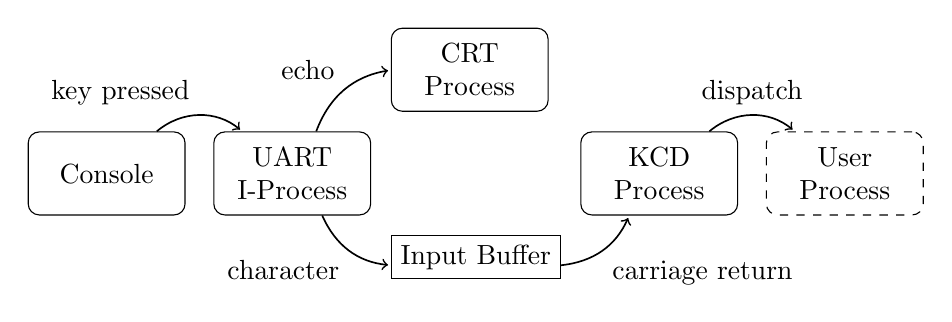
\begin{tikzpicture}[node distance=1em, arrow/.style={->,shorten >=1pt,semithick}, roundedrect/.style={rectangle, draw, text width=5em, text centered, rounded corners, minimum height=3em}, line/.style={draw}, box/.style={draw, rectangle}]
        
        \node [roundedrect] (console) {Console};
        \node [roundedrect, right = of console] (uart) {UART I-Process};
        \node [roundedrect, above right = of uart] (crt) {CRT Process};
        \node [box, below right = of uart] (input) {Input Buffer};
        \node [roundedrect, above right = of input] (kcd) {KCD Process};
        \node [roundedrect, right = of kcd, dashed] (user) {User Process};
        
        \draw[arrow] (console) to[bend left = 40] node[above left] {key pressed} (uart);
        \draw[arrow] (uart) to[bend left] node[above left] {echo} (crt);
        \draw[arrow] (uart) to[bend right] node[below left] {character} (input);
        \draw[arrow] (input) to[bend right] node[below right] {carriage return} (kcd);
        \draw[arrow] (kcd) to[bend left = 40] node[above] {dispatch} (user);
        
    \end{tikzpicture}
    
    \vspace{1em}
    
\end{figure}

\begin{figure}
    
    \centering
    
    \caption{Data Flow of Output Characters}
    \label{fig:outputdataflow}
    
    \vspace{1em}
    
    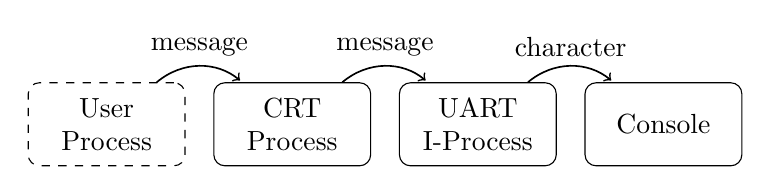
\begin{tikzpicture}[node distance=1em, arrow/.style={->,shorten >=1pt,semithick}, roundedrect/.style={rectangle, draw, text width=5em, text centered, rounded corners, minimum height=3em}, line/.style={draw}, box/.style={draw, rectangle}]
        
        \node [roundedrect, dashed] (user) {User Process};
        \node [roundedrect, right = of user] (crt) {CRT Process};
        \node [roundedrect, right = of crt] (uart) {UART I-Process};
        \node [roundedrect, right = of uart] (console) {Console};
        
        \draw[arrow] (user) to[bend left = 40] node[above] {message} (crt);
        \draw[arrow] (crt) to[bend left = 40] node[above] {message} (uart);
        \draw[arrow] (uart) to[bend left = 40] node[above] {character} (console);
        
    \end{tikzpicture}
    
    \vspace{1em}
    
\end{figure}

\section{System Processes}

\subsection{Null Process}

The \hyperref[alg:nullprocess]{null process} has the lowest priority of any process in the operating system. Since the processor must always be busy, the null process acts as a fail­-safe for situations when no other process can be executed. As such, the null process simply invokes \hyperref[alg:releasingtheprocessor]{\texttt{release_processor}} in an infinite loop.\\

\begin{algorithm}
\caption{Null Process}
\label{alg:nullprocess}
\begin{algorithmic}[1]
\Procedure {null_proc}{\null}
    \While{true}
        \State \Call{release_processor}{\null}
    \EndWhile
\EndProcedure
\end{algorithmic}
\end{algorithm}

\subsection{KCD Process}

The \hyperref[alg:kcdprocess]{Keyboard Command Decoder (KCD) process} provides a console-like interface to users of the operating system. Upon receipt of a command registration message, it uses a global registry to associate the specified command with the message sender. Each time a line of input is entered into the console, the KCD process determines if it is prefixed with a registered command. If so, the input is forwarded to the corresponding process.\\

\begin{algorithm}
\caption{KCD Process}
\label{alg:kcdprocess}
\begin{algorithmic}[1]
\Procedure {kcd_proc}{\null}
    \While{true}
        \State $msg \leftarrow \Call{receive\_message}{sender}$
        \If{$msg.type = \texttt{MSG_TYPE_KCD_REG}$}
            \State $reg \leftarrow$ next unused $kcd\_reg$ entry
            \State $reg.id \leftarrow msg.data$
            \State $reg.pid \leftarrow sender$
        \ElsIf{$msg.type = \texttt{MSG_TYPE_DEFAULT}$}
            \State $id \leftarrow$ first token of $msg.data$
            \If{$kcd\_reg$ contains $id$}
                \State $dispatch\_msg \leftarrow \Call{request\_memory\_block}{\null}$
                \State $dispatch\_msg.type \leftarrow \texttt{MSG_TYPE_KCD_DISPATCH}$
                \State $dispatch\_msg.data \leftarrow msg.data$
                \State \Call{send_message}{$kcd\_reg[id].pid$, $dispatch\_msg$}
            \EndIf
        \EndIf
        \State \Call{release_memory_block}{$msg$}
    \EndWhile
\EndProcedure
\end{algorithmic}
\end{algorithm}

\subsection{CRT Process}

The \hyperref[alg:crtprocess]{CRT process} forwards text to the system console. In order to achieve this, it repeatedly forwards received messages to the UART i-process. It then triggers a UART output interrupt so that the UART i-process may execute. The mechanism by which the UART i-process achieves interrupt-driven output is outlined in \hyperref[subsec:UART I-Process]{Section~\ref*{subsec:UART I-Process}}.\\

\begin{algorithm}
\caption{CRT Process}
\label{alg:crtprocess}
\begin{algorithmic}[1]
\Procedure {crt_proc}{\null}
    \While{true}
        \State $msg \leftarrow \Call{receive\_message}{\null}$
        \If{$msg.type = \texttt{MSG_TYPE_CRT_DISP}$}
            \State \Call{send_message}{$uart\_i\_proc$, $msg$}
        \Else
            \State \Call{release_memory_block}{$msg$}
        \EndIf
    \EndWhile
\EndProcedure
\end{algorithmic}
\end{algorithm}

\section{User Processes}

\subsection{Test Processes}

In order to ensure the correct behaviour of our operating system, we use six user-­level test processes to invoke kernel primitives and check for any incorrect results. These test processes use global variables to coordinate with each other and ensure that  our operating system works as expected. Some of the key mechanisms that are tested include preemption, modification of process priority, memory block assignment, interprocess communication, and system processes such as the KCD and CRT processes.

\subsection{Wall Clock Process}

The wall clock process uses \hyperref[alg:sendingdelayedmessages]{\texttt{delayed_send}} to display a digital clock that updates every second. The process sends itself messages with a delay of one second,
triggering ``tick" updates. Each time the clock ticks, a message is sent to the CRT process using \hyperref[alg:sendingmessages]{\texttt{send_message}} to display the current wall clock time. Upon startup, the wall clock process registers three keyboard commands (\texttt{\%WR}, \texttt{\%WS}, \texttt{\%WT}) with the KCD process which allow the time to be set, reset, and stopped.

\subsection{Set Priority Command Process}

Upon startup, this process registers a keyboard command (\texttt{\%C}) with the KCD process. This command is handled by invoking \hyperref[alg:processpriority]{\texttt{set_process_priority}} using the specified process identifier and priority.

\subsection{Stress Test Processes}

When the \texttt{\%Z} command is entered, these processes test the behaviour of the operating system under severe memory constraints. If the operating system is implemented correctly, the message ``Process C" will be printed to the console every 10 seconds. In order to avoid a deadlock, the priority of process C must be greater than or equal to the priority of process A, as it is responsible for periodically releasing memory blocks.

\chapter{Timing Analysis}

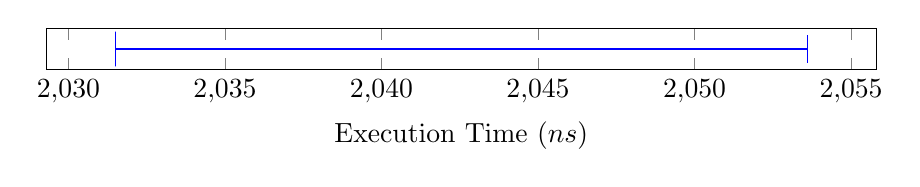
\begin{tikzpicture}
\begin{axis}[height=6em,xlabel=Execution Time ($ns$), max space between ticks=50em,ytick={0}]
    \addplot+[
        boxplot prepared={
            lower whisker=2031.5,
            lower quartile=2031.5,
            median=2031.5,
            upper quartile=2031.5,
            upper whisker=2053.6
        },
    ] coordinates {};
\end{axis}
\end{tikzpicture}

\vspace{3em}

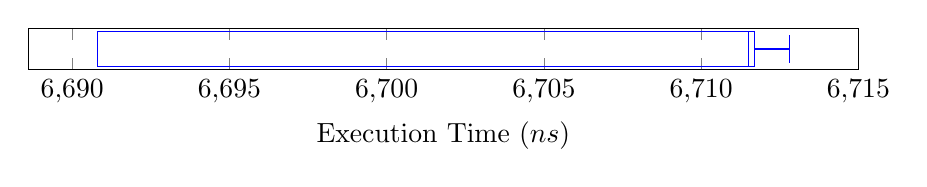
\begin{tikzpicture}
\begin{axis}[height=6em,xlabel=Execution Time ($ns$), max space between ticks=50em,ytick={0}]
    \addplot+[
        boxplot prepared={
            lower whisker=6690.8,
            lower quartile=6690.8,
            median=6711.5,
            upper quartile=6711.7,
            upper whisker=6712.8
        },
    ] coordinates {};
\end{axis}
\end{tikzpicture}

\vspace{3em}

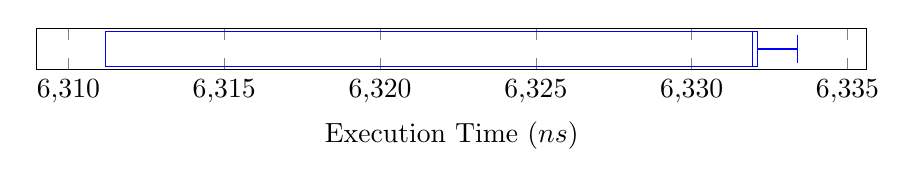
\begin{tikzpicture}
\begin{axis}[height=6em,xlabel=Execution Time ($ns$), max space between ticks=50em,ytick={0}]
    \addplot+[
        boxplot prepared={
            lower whisker=6311.2,
            lower quartile=6311.2,
            median=6331.95,
            upper quartile=6332.1,
            upper whisker=6333.4
        },
    ] coordinates {};
\end{axis}
\end{tikzpicture}

\chapter{Lessons Learned}

\section{Version Control}

At the very beginning of our project, we decided to use \href{http://git-scm.com/}{Git} to manage the source code of our operating system. Paired with \href{http://github.com/}{GitHub}, it provided a robust system for ensuring code quality and minimizing bugs. Throughout the project, we obeyed a strict code review policy; all work was done in individual branches, submitted as a pull request, and then exhaustively reviewed by every member of the team before being merged into the \texttt{master} branch. This policy allowed us to catch several bugs that would have been incredibly difficult to catch in testing.

\section{Simulation}

For the majority of our first deliverable, we tested our operating system exclusively in the debugger provided by the Keil $\mu$Vision IDE. Before submitting the deliverable, we tested our code on the MCB1700 board; everything worked correctly. This substantiated our assumption that the debugger provided a close approximation to the hardware. In reality, as we discovered during our work on the second deliverable, there is a major difference: the SRAM on the MCB1700 board is not initialized the way it is in the debugger. This led to a number of serious bugs that only surfaced when we tested our code on the board. One of the most common bugs involved dealing with strings. Since we relied on the null character to delimit strings, there were portions of code which would work perfectly in the simulator and not on the board. These types of bugs only appeared in the second deliverable, since message passing and console I/O both rely heavily on strings. After dealing with these bugs, we learned to write code more defensively and test our code primarily on the board instead of using the debugger.

\section{Documentation}

Beginning with the first deliverable, we decided to write a portion of our documentation alongside each submission. In the time between the first and third deliverables, we compiled a structural description of each part of our project, wrote pseudocode for each major procedure, and completed most of the Lessons Learned section. This work greatly reduced the amount of time it took to complete our final report, as our documentation was nearly complete by the time we submitted the third deliverable.

\section{Linked Structures}

Early on, we knew that we would need to store data in linked structures for different use cases. Since we wanted to avoid coupling these data structures with the type of data they were storing, we chose to make a generic node structure, \texttt{node_t}:

\begin{minipage}{\textwidth}
\begin{lstlisting}[language=C]
typedef struct node_t {
    struct node_t *mp_next;
    U32 m_val;
} node_t;
\end{lstlisting}
\end{minipage}

We then designed our linked structures to point to nodes of this type. For example, \texttt{queue_t}:

\begin{minipage}{\textwidth}
\begin{lstlisting}[language=C]
typedef struct queue_t {
    node_t *mp_first;
    node_t *mp_last;
} queue_t;
\end{lstlisting}
\end{minipage}

This way, we can declare new node types with additional members for different use cases. For example, here is a process control block:

\begin{minipage}{\textwidth}
\begin{lstlisting}[language=C]
typedef struct k_pcb_t {
    struct k_pcb_t *mp_next;
    U32 *mp_sp;
    U32 m_pid;
    PRIORITY_E m_priority;
    PROC_STATE_E m_state;
    queue_t m_msg_queue;
} k_pcb_t;
\end{lstlisting}
\end{minipage}

As long as the first member is still a pointer to the next node, our linked structures will accommodate these nodes. Creating these generic linked structures saved us a great deal of time in later deliverables.

\section{Data Structure Allocation}

Until the last deliverable, we allocated data structures in the \texttt{memory_init} routine. For example, here is the ready queue:

\begin{minipage}{\textwidth}
\begin{lstlisting}[language=C]
queue_t *gp_ready_queue[NUM_PRIORITIES];

for (i = 0; i < NUM_PRIORITIES; i++) {
    gp_ready_queue[i] = (queue_t *)p_end;
    queue_init(gp_ready_queue[i]);
    p_end += sizeof(queue_t);
}
\end{lstlisting}
\end{minipage}

This approach unnecessarily adds complexity to our code and also led to quite a few time-consuming bugs at the beginning of the project. To fix it, we began to statically allocate our data structures in the operating system image. Here is the same example using static allocation:

\begin{minipage}{\textwidth}
\begin{lstlisting}[language=C]
queue_t g_ready_queue[NUM_PRIORITIES];

for (i = 0; i < NUM_PRIORITIES; i++) {
    queue_init(&g_ready_queue[i]);
}
\end{lstlisting}
\end{minipage}

As a result, our data structures are less error-prone and our code is easier to read. This is the solution that we should have used at the beginning.

\appendix

\addcontentsline{toc}{chapter}{Appendices}
\addtocontents{toc}{\protect\setcounter{tocdepth}{1}}

\chapter{Configuration}
\label{app:configuration}

\section{Parameters}

The following parameters can be adjusted to tune the operating system:\\

\begin{tabularx}{\textwidth}{| l | X |}
    \hline
    \texttt{NUM_BLOCKS} & Number of memory blocks to be placed in the heap.\\
    \hline
    \texttt{BLOCK_SIZE} & Size, in bytes, of each memory block in the heap.\\
    \hline
    \texttt{USR_SZ_STACK} & Size, in bytes, of the stack frame for each process.\\
    \hline
    \texttt{NUM_KCD_REG} & Maximum number of keyboard commands that can be registered using the KCD process.\\
    \hline
    \texttt{KCD_REG_LENGTH} & Maximum length of each command identifier.\\
    \hline
    \texttt{MSG_LOG_SIZE} & Number of recent messages to be logged.\\
    \hline
    \texttt{MSG_LOG_LEN} & Number of characters to be logged for each message.\\
    \hline
    \texttt{NUM_TEST_PROCS} & Number of user test processes.\\
    \hline
\end{tabularx}

\section{Macros}

The following macros can be defined to achieve additional behaviour:\\

\begin{tabularx}{\textwidth}{| l | X |}
    \hline
    \texttt{DEBUG_0} & Allow user test processes to print to the console.\\
    \hline
    \texttt{DEBUG_1} & Enable verbose output for debugging purposes.\\
    \hline
    \texttt{DEBUG_LED} & Monitor the memory heap using the on-board LEDs.\\
    \hline
    \texttt{DEBUG_HOTKEYS} & Enable the debug hotkeys (defined in the README).\\
    \hline
    \texttt{DEBUG_TIMER} & Scale the timer for debugging in the simulator.\\
    \hline
    \texttt{DEBUG_DEMO} & Leave the user test processes in a blocked state.\\
    \hline
\end{tabularx}

\chapter{Global Variables}

\section{Memory}

\subsection{\texttt{g_heap}}

During the memory initialization process, we allocate sections of SRAM into memory blocks. In order to efficiently serve the needs of processes, our operating system uses a linked list to manage these blocks.

\subsection{\texttt{gp_heap_begin_addr}, \texttt{gp_heap_end_addr}}

These variables are set during the memory initialization process and are used for bounds checking in \hyperref[alg:releasingmemoryblocks]{\texttt{release_memory_block}}.

\subsection{\texttt{gp_stack}}

A pointer to the top of the stack. Used during initialization to provide a stack frame for each process.

\section{Processes}

\subsection{\texttt{g_pcbs}}

An array of process control blocks for each process in the system. Indexed by PID for constant time access (e.g., from \hyperref[alg:sendingmessages]{\texttt{send_message}}).

\subsection{\texttt{g_proc_table}}

An array containing the information required (e.g., PID, priority, entry point) to initialize the process control block for each process in the system.

\subsection{\texttt{gp_current_process}}

A pointer to the PCB of the currently executing process. Used mainly for process control purposes (e.g., \hyperref[alg:releasingtheprocessor]{\texttt{release_processor}}).

\subsection{\texttt{g_ready_queue}}

Implemented as an array of queues (one queue for each priority) containing pointers to process control blocks. Used by \hyperref[alg:releasingtheprocessor]{\texttt{release_processor}} for scheduling processes.

\subsection{\texttt{g_blocked_on_memory_queue}}

An array of queues (one queue for each priority) containing pointers to process control blocks. Used by \hyperref[alg:requestingmemoryblocks]{\texttt{request_memory_block}} and \hyperref[alg:releasingmemoryblocks]{\texttt{release_memory_block}} for blocking and unblocking processes.

\subsection{\texttt{g_blocked_on_receive_queue}}

An array of queues (one queue for each priority) containing pointers to process control blocks. Used by \hyperref[alg:sendingmessages]{\texttt{send_message}} and \hyperref[alg:receivingmessages]{\texttt{receive_message}} for blocking and unblocking processes.

\section{Timer I-Process}

\subsection{\texttt{g_timer_count}}
\label{app:gtimercount}

The current system time. Used for determining when delayed messages have expired. Incremented each time a timer interrupt is received (1 ms intervals).

\subsection{\texttt{g_timeout_queue}}
\label{app:gtimeoutqueue}

A queue of messages that have not yet expired. Sorted by expiry time. Used for dispatching delayed messages at the correct time.

\subsection{\texttt{g_timer_preemption_flag}}

Used to indicate whether the timer interrupt handler should preempt the currently executing process on completion of the timer i-process.

\section{UART I-Process}
\label{app:uartglobals}

\subsection{\texttt{g_input_buffer}}

A buffer containing characters that have been entered by the user since the last carriage return.

\subsection{\texttt{g_input_buffer_index}}

The next available index of the input buffer. Incremented each time a character is appended to the input buffer. 

\subsection{\texttt{gp_cur_msg}}

A pointer to the message currently being printed to the console.

\subsection{\texttt{g_output_buffer_index}}

The index of the next character of \texttt{gp_cur_msg} to be printed to the console.

\subsection{\texttt{g_uart_preemption_flag}}

Used to indicate whether the UART interrupt handler should preempt the currently executing process on completion of the UART i-process.

\section{KCD Process}

\subsection{\texttt{g_kcd_reg}}

An array containing keyboard commands that have been registered by other processes (e.g., the wall clock process).

\section{Wall Clock Process}

\subsection{\texttt{g_wall_clock_start_time}}

The system time at which the wall clock was started. Used for computing the elapsed time for display on the console.

\subsection{\texttt{g_wall_clock_start_time_offset}}

The start time specified by the `\texttt{\%WS hh:mm:ss}' command. Used for computing the elapsed time for display on the console.

\subsection{\texttt{g_wall_clock_running}}

A flag used to indicate if the wall clock is currently running. Enables support for pausing and resuming the wall clock.

\end{document}
